\section{Resultados y análisis}

Los datos que se recopilaron para cada muestra y para la interacción con el medio ambiente se muestran en la figura \ref{fig:V_vs_t} junto con la respectiva linealización. 

\begin{figure}[htbp]
    \centering
    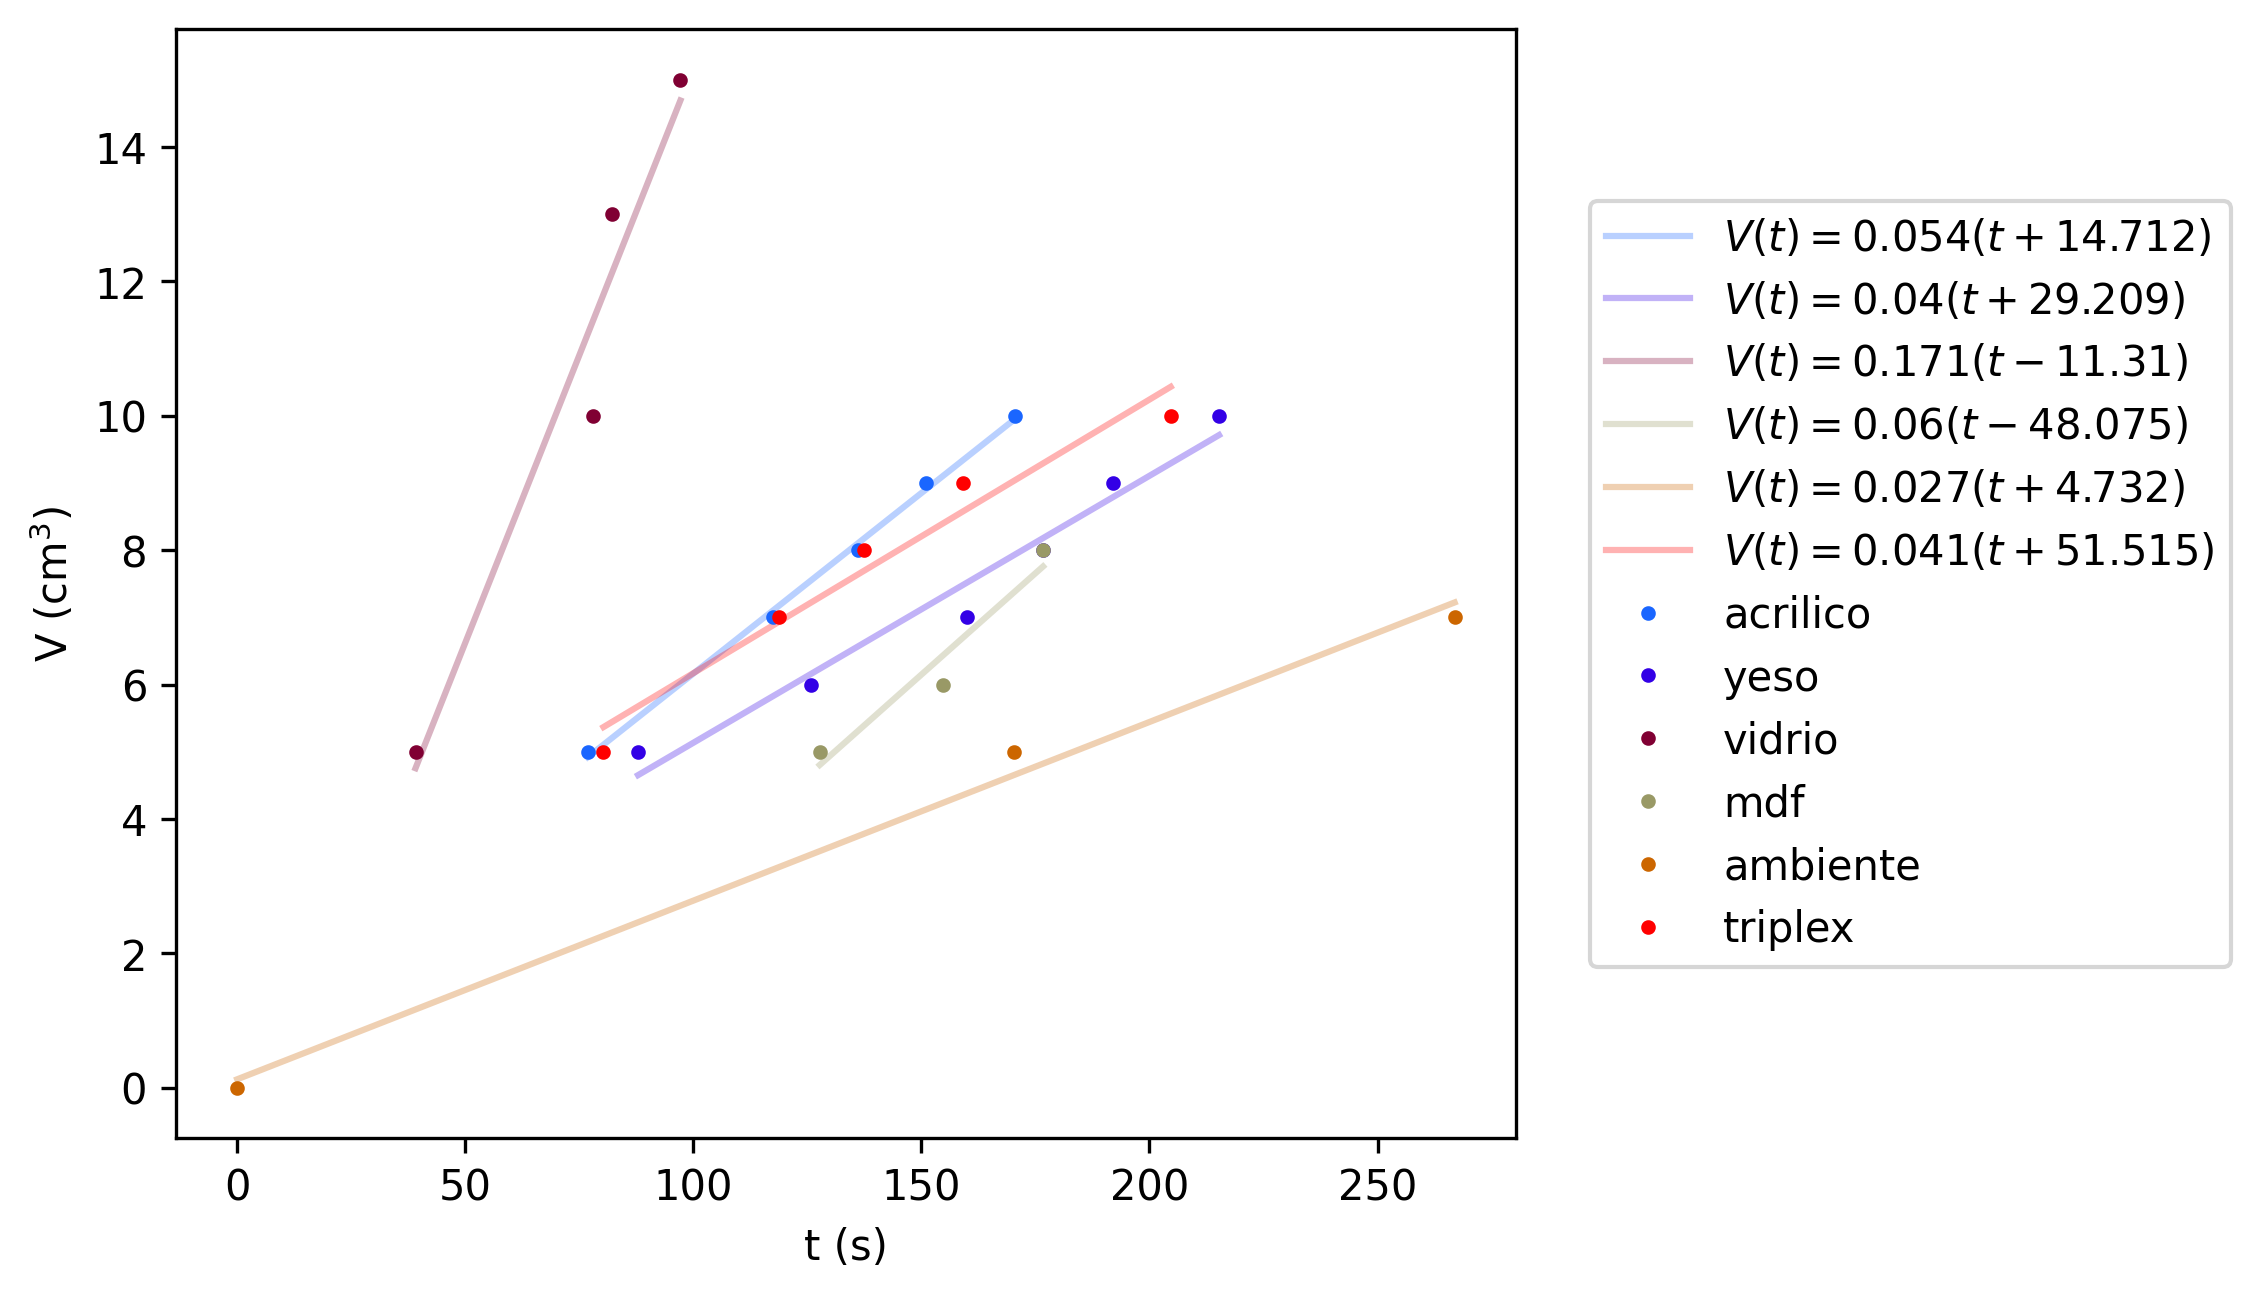
\includegraphics[width=0.5\linewidth]{img/V_vs_t.png}
    \caption{Volumen de hielo fundido como función del tiempo}
    \label{fig:V_vs_t}
\end{figure}

La pendiente que corresponde al intercambio con el medio ambiente, es restada de todas las otras pendientes, de modo que solo se tiene en cuenta la contribución dada por el intercambio de calor con la cámara. El resumen de datos de estas linealizaciones se muestra en la siguiente tabla

\begin{table}[H]
    \centering\begin{tabular}{lSS}
        \toprule
        {Material} & {$\dot V$(\si{\cubic\centi\meter\per\second})} & {$R^2$} \\
        \midrule
        Acrílico & 0.027 & 0.997 \\
        Yeso & 0.013 & 0.968 \\
        Vidrio & 0.145 & 0.949 \\
        MDF & 0.034 & 0.938 \\
        Triplex & 0.014 & 0.959 \\
        \bottomrule
        \end{tabular}
    \caption{Resumen de linealización}
    \label{tab:linealizaciones}
\end{table}

Usando los datos de la tabla \ref{tab:linealizaciones} y la ecuación \eqref{eq:kappa_exp} se calcula la conductividad térmica. Posteriormente, se convirtieron los datos a unidades del sistema internacional ($1\,\si{\calorie_{(4\celsius)}}\si{\per\second\per\centi\meter\per\kelvin} = \SI{419}{\watt\per\meter\per\kelvin}$) para comparar con los datos existentes para las muestras. La comparación se muestra en la tabla \ref{tab:comparacion}
\begin{table}[h]
    \centering
    \begin{tabular}{lSSS}
        \toprule
        {Muestra} & {$\kappa$} & {$\kappa_{\text{ref.}}$} & {e\%} \\
        \midrule
        Triplex & 0.10 & 0.11 & 9.1 \\
        Acrílico & 0.17 & 0.19 & 10.5 \\
        Vidrio & 1.06 & 0.86 & 23.3 \\
        Yeso & 0.08 & 0.43 & 81.4 \\
        MDF & 0.20 & 0.08 & 150.0 \\
        \bottomrule
        \end{tabular}
        \caption{Comparación con los valores conocidos}
        \label{tab:comparacion}
\end{table}